
We tested the regularization strategies presented in Section~\ref{sec:kernel_reg}
in the context of improving generalization on small datasets and training robust models.
Our goal is to use common architectures used for large datasets and improve
their performance in different settings through regularization.
Our Pytorch implementation of the various strategies is available at \url{https://github.com/albietz/kernel_reg}.

For the adversarial training strategies, the inner maximization problems are solved using 5 steps of projected
gradient ascent with constant step-lengths.
In the case of the lower bound penalties $\|f\|_\delta^2$ and~$\|\nabla f\|^2$,
we also maximize over
examples in the mini-batch, only considering the maximal element when computing gradients with respect to parameters.
For the robust optimization problem~\eqref{eq:robust}, we use PGD with~$\ell_2$
perturbations,
as well as the corresponding~$\ell_2$ (squared) gradient norm penalty on the loss.
For the upper bound approaches with spectral norms (SNs), we consider the SN projection strategy with decaying~$\tau$,
as well as the SN penalty~\eqref{eq:optimization_problem_penalized}, either using power iteration (PI) or a full SVD
for computing gradients.



\subsection{Improving generalization on small datasets}
\label{sub:exp_smalldata}
We consider the datasets CIFAR10 and MNIST when using a small number of training examples,
as well as 102 datasets of biological sequences that suffer from small sample size.

\vspace*{-0.2cm}
\paragraph{CIFAR10.}
In this setting, we use 1\,000 and 5\,000 examples of the CIFAR10 dataset, with or without data augmentation.
We consider a VGG network~\citep{simonyan2014very} with 11 layers,
as well as a residual network~\citep{he2016deep} with 18 layers, which achieve
91\% and 93\% test accuracy respectively when trained on the full training set with standard data augmentation (horizontal flips + random crops).
We do not use batch normalization layers in order to prevent any interaction with spectral norms.
Each strategy derived in Section \ref{sec:kernel_reg} is trained for 500 epochs
using SGD with momentum and batch size 128, halving the step-size every 40 epochs.
In order to study the potential effectiveness of each method, we assume that a reasonably large validation set is
available to select hyper-parameters; thus, we keep 10\,000 annotated examples for this purpose.
We also show results using a smaller validation set in Appendix~\ref{sub:cifar_appx}.

\begin{table}[tb]
\caption{Regularization on CIFAR10 with 1\,000 examples for VGG-11 and ResNet-18.
Each entry shows the test accuracy with/without data augmentation when all hyper-parameters are optimized on a validation set.
See also Section~\ref{sub:cifar_appx} in the appendix for additional results and statistical testing.
}

\label{tab:smalldata}
\centering
\small
\vspace{0.2cm}
\begin{tabular}{ | l | c | c |  }
\hline
Method & 1k VGG-11 & 1k ResNet-18 \\ \hline
\hline
No weight decay & 50.70 / 43.75 & 45.23 / 37.12 \\
Weight decay & 51.32 / 43.95 & 44.85 / 37.09 \\
SN penalty (PI) & 54.64 / 45.06 & 47.01 / 39.63 \\
SN projection & 54.14 / \textbf{\color{darkgray}46.70} & 47.12 / 37.28 \\
VAT & 50.88 / 43.36 & 47.47 / 42.82 \\
PGD-$\ell_2$ & 51.25 / 44.40 & 45.80 / 41.87 \\
grad-$\ell_2$ & \textbf{\color{darkgray}55.19} / 43.88 & \textbf{49.30} / \textbf{\color{darkgray}44.65} \\
\hline
$\|f\|_\delta^2$ penalty & 51.41 / 45.07 & 48.73 / 43.72 \\
$\|\nabla f\|^2$ penalty & 54.80 / 46.37 & \textbf{\color{darkgray}48.99} / \textbf{44.97} \\
PGD-$\ell_2$ + SN proj & 54.19 / \textbf{\color{darkgray}46.66} & 47.47 / 41.25 \\
grad-$\ell_2$ + SN proj & \textbf{55.32} / \textbf{46.88} & 48.73 / 42.78 \\
$\|f\|_\delta^2$ + SN proj & 54.02 / \textbf{\color{darkgray}46.72} & 48.12 / 43.56 \\
$\|\nabla f\|^2$ + SN proj & \textbf{55.24} / \textbf{46.80} & \textbf{\color{darkgray}49.06} / \textbf{44.92} \\
\hline
\end{tabular}
\end{table}

Table~\ref{tab:smalldata} shows the test accuracies on 1\,000 examples for upper and lower bound approaches,
as well as combined ones.
We also include virtual adversarial training~\citep[VAT,][]{miyato2018virtual}.
We provide extended tables in Appendix~\ref{sub:cifar_appx} with additional methods,
other geometries, results for 5\,000 examples, as well as hypothesis tests for
comparing pairs of methods and assessing the significance of our findings.
Overall, we find that the combined lower bound + SN constraints approaches often
yield better results than either method separately.
For lower bound approaches alone, we found our $\|f\|_\delta^2$ and~$\|\nabla f\|^2$ penalties to often
work best, particularly without data augmentation,
while robust optimization strategies can be preferable with data augmentation,
perhaps thanks to the adaptive regularization effect discussed earlier, which may be helpful in
this easier setting.
Gradient penalties often outperform adversarial perturbation strategies,
possibly because of the closed form gradients which may improve optimization.
We also found that adversarial training strategies tend to poorly control SNs compared to
gradient penalties, particularly PGD (see also Section~\ref{sub:exp_robust}).
SN constraints alone can also work well in some cases, particularly for VGG architectures,
and often outperform SN penalties.
SN penalties can work well nevertheless and provide computational benefits when using the power iteration variant.


\begin{table}[tb]
\caption{Regularization on 300 or 1\,000 examples from MNIST, using deformations from Infinite MNIST.
($\ast$) indicates that random deformations were included as training examples,
while $\|f\|_\tau^2$ and $\|D_\tau f\|^2$
use them as part of the regularization penalty. 
See Section~\ref{sub:imnist_appx} in the appendix for more results and statistical testing.
}

\label{tab:imnist}
\centering
\small
\vspace{0.2cm}
% python print_table_imnist.py --lr --paper
\begin{tabular}{ | l | c | c |  }
\hline
Method & 300 VGG & 1k VGG \\ \hline
\hline
Weight decay & 89.32 & 94.08 \\
SN projection & 90.69 & 95.01 \\
grad-$\ell_2$ & 93.63 & 96.67 \\
$\|f\|_\delta^2$ penalty & 94.17 & 96.99 \\
$\|\nabla f\|^2$ penalty & 94.08 & 96.82 \\
\hline
Weight decay ($\ast$) & 92.41 & 95.64 \\
grad-$\ell_2$ ($\ast$) & 95.05 & 97.48 \\
\hline
$\|D_\tau f\|^2$ penalty & 94.18 & 96.98 \\
$\|f\|_\tau^2$ penalty & 94.42 & 97.13 \\
$\|f\|_{\tau}^2$ + $\|\nabla f\|^2$ & 94.75 & 97.40 \\
$\|f\|_{\tau}^2$ + $\|f\|^2_\delta$ & 95.23 & \textbf{\color{darkgray}97.66} \\
$\|f\|_{\tau}^2$ + $\|f\|^2_\delta$ ($\ast$) & \textbf{95.53} & \textbf{\color{darkgray}97.56} \\
$\|f\|_{\tau}^2$ + $\|f\|^2_\delta$ + SN proj & 95.20 & \textbf{\color{darkgray}97.60} \\
$\|f\|_{\tau}^2$ + $\|f\|^2_\delta$ + SN proj ($\ast$) & \textbf{\color{darkgray}95.40} & \textbf{97.77} \\
\hline
\end{tabular}
% \vspace*{-0.1cm}
\end{table}

\vspace*{-0.2cm}
\paragraph{Infinite MNIST.}
In order to assess the effectiveness of lower bound penalties based on deformation stability,
we consider the Infinite MNIST dataset~\citep{loosli-canu-bottou-2006}, which provides an ``infinite''
number of transformed generated examples for each of the 60\,000 MNIST training digits.
Here, we use a 5-layer VGG-like network with average pooling after each 3x3 convolution layer,
in order to more closely match the architecture assumptions of~\citet{bietti2018group}
for deformation stability.
We consider two lower bound penalties that leverage the digit transformations in Infinite MNIST:
one based on ``adversarial'' deformations around each digit, denoted~$\|f\|_\tau^2$;
and a tangent propagation~\citep{simard1998transformation} variant, denoted $\|D_\tau f\|^2$,
which provides an approximation to~$\|f\|_\tau^2$ for small deformations
based on gradients along a few tangent vector directions given by deformations
(see Appendix~\ref{sec:deformation_penalties} for details).
Table~\ref{tab:imnist} shows the obtained test accuracy for subsets of MNIST of size 300 and 1\,000.
Overall, we find that combining both adversarial penalties $\|f\|_\tau^2$ and $\|f\|_\delta^2$
performs best, which suggests that it is helpful to obtain tighter lower approximations of the RKHS
norm by considering perturbations of different kinds.
Explicitly controlling the spectral norms can further improve performance,
as does training on deformed digits, which may yield better margins
by exploiting the additional knowledge that small deformations preserve labels.
Note that data augmentation alone (with some weight decay) does quite poorly in this case,
even compared to our lower bound penalties which do not use deformations.


\begin{table}[tb]
\caption{Regularization on protein homology detection tasks,
with or without data augmentation (DA).
Fixed hyperparameters are selected using the first half of the datasets,
and we report the average auROC50 score on the second half.
See Section~\ref{sub:protein_appx} in the appendix for more details and statistical testing.
}

\label{tab:protein}
\centering
\small
\vspace{0.2cm}
\begin{tabular}{|l|c|c|}
\hline
 Method                       &   No DA &    DA \\ \hline
\hline
 No weight decay              &   0.421 & 0.541 \\
 Weight decay                 &   0.432 & 0.544 \\
 SN proj                      &   0.583 & 0.615 \\
 PGD-$\ell_2$                 &   0.488 & 0.554 \\
 grad-$\ell_2$                &   0.551 & 0.570 \\ \hline
 $\|f\|_{\delta}^2$           &   0.577 & 0.611 \\
 $\|\nabla f\|^2$             &   0.566 & 0.598 \\
 PGD-$\ell_2$ + SN proj       &   \textbf{\color{darkgray}0.615} & \textbf{\color{darkgray}0.622} \\
 grad-$\ell_2$ + SN proj      &   0.581 & \textbf{\color{darkgray}0.634} \\
 $\|f\|_{\delta}^2$ + SN proj &   \textbf{0.631} & \textbf{0.639} \\
 $\|\nabla f\|^2$ + SN proj   &   0.576 & \textbf{\color{darkgray}0.617} \\
\hline
\end{tabular}
\vspace*{-0.1cm}
\end{table}

\vspace{-0.2cm}
\paragraph{Protein homology detection.}
Remote homology detection between protein sequences is an important problem to understand protein structure.
Given a protein sequence, the goal is to predict whether it belongs to a superfamily of interest.
We consider the Structural Classification Of Proteins (SCOP) version 1.67 dataset~\citep{murzin1995scop},
which we process as described in Appendix~\ref{sub:protein_appx}
in order to obtain 102 balanced binary classification tasks with 100 protein sequences each,
thus resulting in a low-sample regime. Protein sequences were also cut to $400$ amino acids.

Sequences are represented with a one-hot encoding strategy---that is, a
sequence of length~$l$ is represented as a binary matrix in $\{0,1\}^{20 \times
l}$, where $20$ is the number of different amino acids (alphabet size of the sequences).
Such a structure can then be processed by convolutional neural
networks~\citep{alipanahi2015predicting}.
In this paper, we do not try to optimize the structure of the network for the task,
since our goal is only to evaluate the effect of regularization strategies.
Therefore, we use a simple convolutional network with 3 convolutional layers
followed by global max-pooling and a final fully-connected layer
(we use filters of size 5, and a max-pooling layer after the second convolutional layer).

Training was done using Adam with a learning rate fixed to $0.01$, and a weight decay parameter
tuned for each method.
Since hyper-parameter selection per dataset is difficult due to the low sample size, we use the
same parameters across datasets. This allows us
to use the first 51 datasets as a validation set for hyper-parameter tuning,
and we report average performance with these fixed choices on the remaining 51 datasets.
The standard performance measure for this task is the auROC50 score (area under the ROC curve up to 50\% false positives).
We note that the selection of  hyper-parameters has a transductive component, since some of the sequences
in the test datasets may also appear in the datasets used for validation (possibly with a different label).

The results are shown in Table~\ref{tab:protein}.
The procedure used for data augmentation (right column) is described in Appendix~\ref{sub:protein_appx}.
We found that the most effective approach is the adversarial perturbation penalty,
together with SN constraints.
In particular, we found it to outperform the gradient penalty~$\|\nabla f\|^2$,
perhaps because in this case gradient penalties are only computed on a discrete set
of possible points given by one-hot encodings, while adversarial perturbations may
increase stability to wider regions, potentially covering different possible encoded
sequences.




\subsection{Training adversarially robust models}
\label{sub:exp_robust}

\begin{figure}[tb]
	\centering
	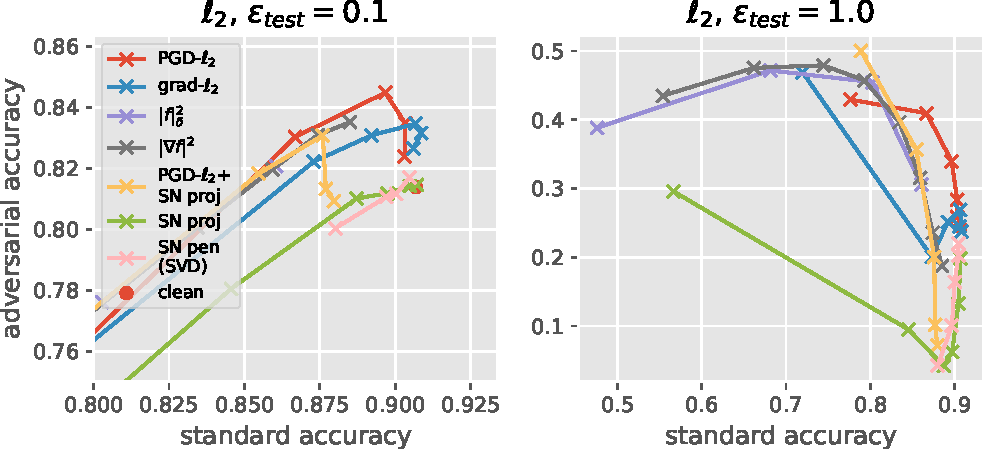
\includegraphics[width=.95\columnwidth]{figures/cifar10_vgg/test_vs_adv_l2_comp.pdf}
        \vspace*{-0.1cm}
	\caption{Robustness trade-off curves of different regularization methods for VGG11 on CIFAR10.
	Each plot shows test accuracy vs adversarial test accuracy
	for $\ell_2$-bounded, 40-step PGD adversaries with a fixed~$\epsilon_{\text{test}}$.
	Different points on a curve correspond to training with different regularization strengths.
	The regularization increases monotonically along a given curve, and
	the leftmost points correspond to the strongest regularization.
	For PGD-$\ell_2$ + SN projection, we vary~$\epsilon$ with a fixed~$\tau = 0.8$.
	}
	\label{fig:robust_tradeoffs}
        \vspace*{-0.2cm}
\end{figure}

We consider the same VGG architecture as in Section~\ref{sub:exp_smalldata}, trained on CIFAR10
with data augmentation, with different regularization strategies.
Each method is trained for 300 epochs using SGD with momentum and batch size 128, dividing the step-size in half every 30 epochs.
This strategy was successful in reaching convergence for all methods.

Figure~\ref{fig:robust_tradeoffs} shows the test accuracy of the different methods in the presence
of $\ell_2$-bounded adversaries, plotted against standard accuracy.
We can see that the robust optimization approaches tend to work better in high-accuracy regimes, perhaps because the local stability that they encourage is sufficient on this dataset,
while the~$\|f\|_\delta^2$
penalty can be useful in large-perturbation regimes.
We find that upper bound approaches alone do not provide robust models,
but combining the SN constraint approach with a lower bound strategy
(in this case PGD-$\ell_2$) helps improve robustness perhaps thanks to a more explicit control of stability.
The plots also confirm that gradient penalties on the loss may be preferable for small regularization strengths (they achieve higher accuracy while improving robustness for small~$\epsilon_{test}$),
while for stronger regularization,
the gradient approximation no longer holds and the adversarial training approaches such
as PGD (and its combination with SN constraints) are preferred.
More experiments confirming these findings are available in Section~\ref{sub:robustness_appx} of the appendix.

\begin{figure}[tb]
%run margin_plots.py --experiment cifar10_vgg  --jacobianl2max --norm kernel_multi --reload --xlim "-1 15" --paper
	\centering
	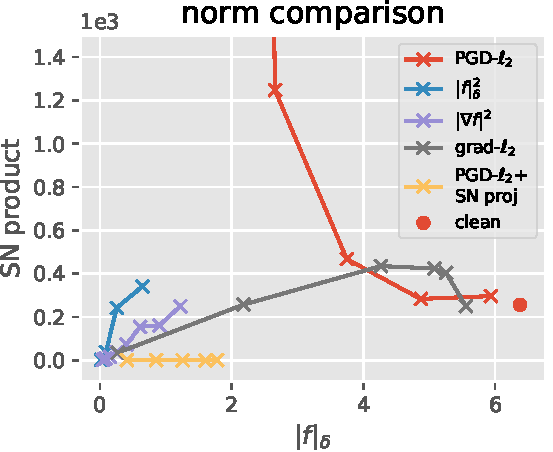
\includegraphics[width=.48\columnwidth]{figures/cifar10_vgg/norm_comp_sn_prod.pdf}% ~~~~~ \\
	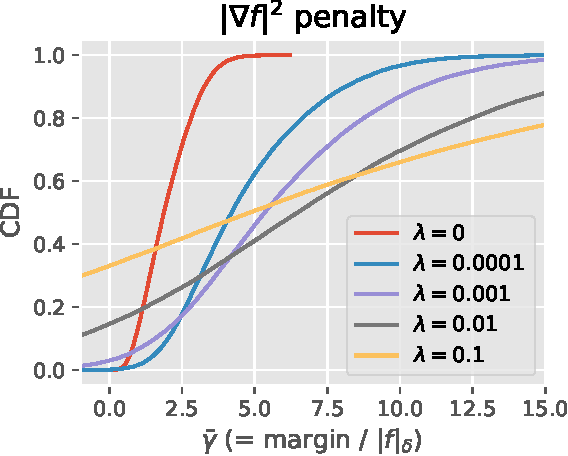
\includegraphics[width=.48\columnwidth]{figures/cifar10_vgg/jacobianl2max_margins_kernel_multi.pdf}
        \vspace*{-0.1cm}
	\caption{(left) Comparison of lower and upper bound quantities ($\|f\|_\delta$ vs the product of spectral norms).
	(right) CDF plot of normalized empirical margins for the $\|\nabla f\|^2$ penalty with different
	regularization strengths, normalized by $\|f\|_\delta$.
	We consider 1000 fixed training examples when computing $\|f\|_\delta$.}
        \vspace*{-0.2cm}
	\label{fig:norms_and_margins}
\end{figure}

\vspace*{-0.2cm}
\paragraph{Norm comparison and adversarial generalization.}
Figure~\ref{fig:norms_and_margins} (left) compares lower and upper bound quantities
for different regularization strengths.
Note that for PGD, in contrast to other methods, we can see that the product of spectral norms (representative of an upper bound on~$\|f\|_\Hc$) increases when the lower bound~$\|f\|_\delta$ decreases.
This suggests that a network learned with PGD with large~$\epsilon$ may have large RKHS norm, possibly because the approach
tries to separate $\epsilon$-balls around the training examples,
which may require a more complex model than simply separating the training
examples~\citep[see also][]{madry2018towards}.
This large discrepancy between upper and lower bounds highlights the fact that such models may only
be stable locally near training data, though this happens to be enough for robustness on many test examples on CIFAR10.

In contrast, for other methods, and in particular the lower bound penalties~$\|f\|_\delta^2$ and~$\|\nabla f\|^2$,
the upper and lower bounds appear more tightly controlled, suggesting a more appropriate control
of the RKHS norm.
This makes our guarantees on adversarial generalization more meaningful,
and thus we may look at the empirical
distributions of normalized margins~$\bar{\gamma}$ obtained using $\|f\|_\delta$ for normalization (as an approximation of~$\|f\|_\Hc$),
shown in Figure~\ref{fig:norms_and_margins} (right).
The curves suggest that for small~$\bar{\gamma}$, and hence small $\epsilon_{test}$,
smaller values of~$\lambda$ are preferred, while stronger regularization helps
for larger~$\bar \gamma$, yielding lower test error guarantees in the presence of stronger adversaries
according to our bounds in
Section~\ref{sub:guarantees}.
This qualitative behavior is indeed observed in the results of Figure~\ref{fig:robust_tradeoffs} on test data
for the $\|\nabla f\|^2$ penalty.

